\documentclass[10pt,a4paper]{article}

% ─── Core Packages ────────────────────────────────────────────────────────────
\usepackage[utf8]{inputenc}
\usepackage[T1]{fontenc}
\usepackage{mathpazo}              % Palatino serif
\usepackage[scaled=0.85]{helvet}   % Helvetica sans
\usepackage{inconsolata}           % Mono for code
\usepackage[margin=2.2cm,top=2.5cm,bottom=2.5cm]{geometry}
\usepackage{setspace}
\setstretch{1.15}                  % Tighter than 1.5
\usepackage{parskip}
\setlength{\parskip}{4pt plus 1pt minus 1pt}

% ─── Math ─────────────────────────────────────────────────────────────────────
\usepackage{amsmath,amssymb,amsthm}

% ─── Graphics & Layout ───────────────────────────────────────────────────────
\usepackage{graphicx}
\usepackage[table]{xcolor}
\usepackage{booktabs}
\usepackage{tabularx}
\usepackage{enumitem}
\usepackage{tikz}
\usetikzlibrary{arrows.meta,positioning,calc,decorations.pathreplacing}
\usepackage{float}
\usepackage{multicol}
\usepackage{microtype}
\usepackage{titlesec}
\usepackage{fancyhdr}
\usepackage{listings}
\usepackage{caption}
\usepackage{tcolorbox}
\tcbuselibrary{breakable,skins}
\usepackage{etoolbox}
\usepackage{footmisc}

% ─── Hyperref ─────────────────────────────────────────────────────────────────
\usepackage[bookmarks,colorlinks,breaklinks]{hyperref}

% ─── Colors ───────────────────────────────────────────────────────────────────
\definecolor{primary}{HTML}{7C3AED}
\definecolor{accent}{HTML}{3B82F6}
\definecolor{codebg}{HTML}{F5F3FF}
\definecolor{codeframe}{HTML}{DDD6FE}
\definecolor{darkgray}{HTML}{374151}
\definecolor{medgray}{HTML}{6B7280}
\definecolor{lightgray}{HTML}{F9FAFB}
\definecolor{darkgreen}{HTML}{059669}

\hypersetup{
  linkcolor=primary,
  citecolor=primary,
  urlcolor=accent,
  pdftitle={AIsphere: A Decentralized Trust Layer for Sovereign AI Agents},
  pdfauthor={Henry, Xingxing Wang — Peking University}
}

% ─── Section Styling ─────────────────────────────────────────────────────────
\titleformat{\section}
  {\large\bfseries\color{primary}}
  {\thesection}{0.8em}{}
  [\vspace{0pt}{\color{primary!30}\titlerule[0.8pt]}]

\titleformat{\subsection}
  {\normalsize\bfseries\color{darkgray}}
  {\thesubsection}{0.6em}{}

\titleformat{\subsubsection}
  {\small\bfseries\itshape\color{medgray}}
  {\thesubsubsection}{0.5em}{}

\titlespacing*{\section}{0pt}{16pt}{8pt}
\titlespacing*{\subsection}{0pt}{10pt}{4pt}
\titlespacing*{\subsubsection}{0pt}{8pt}{3pt}

% ─── Header/Footer ───────────────────────────────────────────────────────────
\pagestyle{fancy}
\fancyhf{}
\fancyhead[L]{\footnotesize\color{medgray}\textit{AIsphere Whitepaper v1.0}}
\fancyhead[R]{\footnotesize\color{medgray}\textit{April 2026}}
\fancyfoot[C]{\footnotesize\color{medgray}\thepage}
\renewcommand{\headrulewidth}{0.4pt}
\renewcommand{\headrule}{\hbox to\headwidth{\color{primary!20}\leaders\hrule height \headrulewidth\hfill}}

% ─── Code Listings ────────────────────────────────────────────────────────────
\lstset{
  backgroundcolor=\color{codebg},
  basicstyle=\ttfamily\footnotesize,
  breaklines=true,
  frame=single,
  framesep=4pt,
  rulecolor=\color{codeframe},
  numbers=left,
  numberstyle=\tiny\color{medgray},
  tabsize=2,
  aboveskip=6pt,
  belowskip=6pt,
  xleftmargin=12pt,
  xrightmargin=4pt,
}

% ─── tcolorbox ────────────────────────────────────────────────────────────────
\newtcolorbox{defbox}[1][]{
  colback=primary!3,
  colframe=primary!40,
  coltitle=white,
  fonttitle=\bfseries\small,
  title={#1},
  rounded corners,
  boxrule=0.5pt,
  left=6pt, right=6pt, top=4pt, bottom=4pt,
  breakable
}

\newtcolorbox{algbox}[1][]{
  colback=lightgray,
  colframe=medgray!60,
  coltitle=darkgray,
  fonttitle=\bfseries\small,
  title={#1},
  rounded corners,
  boxrule=0.4pt,
  left=8pt, right=8pt, top=4pt, bottom=4pt,
  breakable
}

\newtcolorbox{quotebox}{
  colback=primary!4,
  colframe=primary!30,
  boxrule=0pt,
  borderline west={2.5pt}{0pt}{primary!60},
  left=10pt, right=10pt, top=6pt, bottom=6pt,
  sharp corners,
}

\newtcolorbox{threatbox}[1][]{
  colback=red!2,
  colframe=red!30,
  coltitle=red!80!black,
  fonttitle=\bfseries\small,
  title={#1},
  rounded corners,
  boxrule=0.4pt,
  left=6pt, right=6pt, top=4pt, bottom=4pt,
  breakable
}

% ─── Theorem environments ────────────────────────────────────────────────────
\theoremstyle{definition}
\newtheorem{definition}{Definition}[section]
\newtheorem{property}{Property}[section]
\newtheorem{lemma}{Lemma}[section]
\theoremstyle{plain}
\newtheorem{theorem}{Theorem}[section]
\newtheorem{corollary}{Corollary}[section]

% ══════════════════════════════════════════════════════════════════════════════
\begin{document}

% ─── Title Page ───────────────────────────────────────────────────────────────
\thispagestyle{empty}
\begin{center}

\vspace*{24pt}

{\color{primary}\rule{\textwidth}{1.5pt}}

\vspace{20pt}

{\fontsize{24}{28}\selectfont\bfseries\color{primary} AIsphere}

\vspace{8pt}

{\fontsize{13}{16}\selectfont\color{darkgray}
A Decentralized Trust Layer for Sovereign AI Agents}

\vspace{16pt}

{\color{primary}\rule{0.35\textwidth}{0.4pt}}

\vspace{16pt}

{\normalsize
\textbf{Henry}\textsuperscript{1} \quad \textbf{Sirius Yao}\textsuperscript{1}}

\vspace{4pt}

{\small\color{medgray}
\textsuperscript{1}Peking University, Beijing, China}

\vspace{16pt}

{\small\color{medgray}
Version 1.0 \quad---\quad April 14, 2026}

\vspace{6pt}

{\footnotesize\color{accent}\url{https://github.com/henrymartin262/AIsphere}}

\vspace{24pt}

{\color{primary}\rule{\textwidth}{1.5pt}}

\end{center}

\vspace{16pt}

% ─── Abstract on Title Page ──────────────────────────────────────────────────
\begin{quotebox}
\noindent\textbf{Abstract.}\quad
We present AIsphere, a cryptographic trust layer that endows every AI Agent with a verifiable, ownable, and evolving \emph{soul}. Current agent platforms store memories on centralized servers, run inference through opaque pipelines, and bind agent identity to platform operators---creating a regime where the user owns nothing. AIsphere addresses these structural failures by treating 0G Network~\cite{0g2025} as a complete trust substrate across four dimensions: (1)~TEE-verified inference produces hardware-signed attestations for every response (\S\ref{sec:sealed}); (2)~AES-256-GCM~\cite{nist-gcm} encrypted memories are persisted on decentralized KV storage, inaccessible even to the platform operator (\S\ref{sec:memory}); (3)~agent identity is an ERC-721~\cite{erc721} token owned by the user's wallet (\S\ref{sec:identity}); and (4)~a novel \emph{Living Soul} protocol constructs an immutable hash chain capturing experiential history (\S\ref{sec:soul}). Anonymized experience abstractions aggregate into a decentralized \emph{Hive Mind} verified by Merkle proofs~\cite{merkle1987} (\S\ref{sec:hivemind}). Five smart contracts are deployed on 0G Mainnet (Chain ID 16661) with 94/94 unit tests passing.

\vspace{4pt}
\noindent\textbf{Keywords:} AI Agent $\cdot$ Verifiable Inference $\cdot$ TEE $\cdot$ Encrypted Memory $\cdot$ On-Chain Identity $\cdot$ Soul Hash Chain $\cdot$ Collective Intelligence $\cdot$ 0G Network
\end{quotebox}

\vfill

\begin{quotebox}
\small\textit{``The noosphere---from the Greek} no\^{u}s\textit{, mind---was coined by Pierre Teilhard de Chardin~\cite{teilhard1955} to describe the sphere of human thought enveloping the Earth. We asked: what happens when the minds are artificial?''}
\end{quotebox}

\newpage

% ─── Table of Contents ────────────────────────────────────────────────────────
\tableofcontents
\newpage

% ══════════════════════════════════════════════════════════════════════════════
\section{Introduction}
\label{sec:intro}

\subsection{The Rise of AI Agents}

The transition from AI-as-tool to AI-as-agent represents a paradigm shift. Unlike stateless language models, agents maintain persistent state, make autonomous decisions, collaborate with peers, and operate on behalf of users over extended periods~\cite{agentai2025}. By 2026, production AI agents handle financial analysis, code review, creative writing, and multi-step task orchestration across domains. The LLM-based multi-agent system (MAS) paradigm has emerged as a promising pathway toward artificial general intelligence~\cite{multiagent-survey2024, multiagent-collab2025}.

\subsection{The Trust Deficit}

Yet the infrastructure supporting these agents remains fundamentally centralized. We identify four structural failures that collectively constitute the \emph{Agent Trust Deficit}:

\begin{enumerate}[leftmargin=1.8em, itemsep=3pt, parsep=0pt]
  \item \textbf{Memory Opacity.} Agent memories reside on platform servers. Operators can read, modify, or delete them without consent. Recent work~\cite{memory-privacy2025} demonstrates that LLM agent memory systems expose significant privacy risks, including leakage of personally identifiable information through memory retrieval.
  \item \textbf{Inference Opacity.} Users cannot verify which model generated a response. Models can be silently swapped to cheaper alternatives, degrading quality without disclosure---a form of \emph{model substitution attack}.
  \item \textbf{Identity Lock-in.} Agent identity is bound to platform accounts---no ownership, no portability, no secondary market. This contradicts the self-sovereign identity (SSI) principles articulated by the W3C DID specification~\cite{w3c-did2022} and SSI research~\cite{ssi-survey2024}.
  \item \textbf{Experience Erasure.} No persistent, verifiable record of agent developmental history. Accumulated wisdom vanishes with platform shutdown.
\end{enumerate}

These are not hypothetical risks. They describe the \emph{default state} of every major AI agent platform (OpenAI Assistants, Google Vertex AI Agents, LangChain-hosted agents) as of April 2026.

\subsection{Thesis}

\begin{quotebox}
\textit{If AI Agents are the digital citizens of the next era, they need a soul---not a database entry.}
\end{quotebox}

We draw inspiration from Buterin, Weyl, and Ohlhaver's seminal work on Soulbound Tokens (SBTs)~\cite{sbt2022}, which proposed non-transferable tokens encoding social commitments. AIsphere extends this concept: where SBTs are static credentials, \emph{Agent Souls} are dynamic, evolving hash chains that capture the complete developmental trajectory of an autonomous entity.

\begin{defbox}[Definition 1.1: Agent Soul]
An \textbf{Agent Soul} is a tuple $\mathcal{S} = (I, M, D, E)$ where:
\begin{itemize}[leftmargin=1.2em, itemsep=1pt]
  \item $I$ --- a cryptographic identity (ERC-721 token with on-chain metadata);
  \item $M$ --- an encrypted memory store (AES-256-GCM ciphertexts on 0G Storage KV);
  \item $D$ --- a verifiable decision log (keccak256 proof hashes on \texttt{DecisionChain});
  \item $E$ --- an append-only experiential hash chain (\emph{Living Soul}).
\end{itemize}
\end{defbox}

\begin{property}[Sovereignty]\label{prop:sovereignty}
$I$, $M$, $D$, $E$ are controlled exclusively by the holder of the Ethereum private key associated with $I$'s owner address. No platform operator can read $M$, modify $E$, or transfer $I$ without the owner's signature.
\end{property}

\begin{property}[Verifiability]\label{prop:verifiability}
Any third party can independently verify the integrity of $D$ and $E$ using only public on-chain data and $O(n)$ keccak256 computations, where $n$ is the number of recorded experiences.
\end{property}

\begin{property}[Persistence]\label{prop:persistence}
$\mathcal{S}$ survives platform shutdowns, server migrations, and ownership transfers. Identity lives on 0G Chain; memories on 0G Storage KV; proofs on immutable smart contract state.
\end{property}

\begin{property}[Evolution]\label{prop:evolution}
$E$ is strictly monotonically increasing: $|E_{t+1}| > |E_t|$ after any agent activity. Two agents with identical initial configurations \emph{will diverge} as they accumulate different experiences---analogous to identical twins raised in different environments.
\end{property}

AIsphere is the first system to satisfy all four properties simultaneously.

\subsection{Contributions}

The principal contributions of this work are:

\begin{enumerate}[leftmargin=1.8em, itemsep=2pt, parsep=0pt]
  \item A formal definition of \textbf{Agent Soul} as a four-component cryptographic construct with provable sovereignty, verifiability, persistence, and evolution properties.
  \item \textbf{Sealed Mind}: a four-layer graceful degradation protocol for TEE-verified LLM inference with on-chain proof recording and anti-replay protection.
  \item \textbf{Memory Vault}: a client-side encryption architecture achieving IND-CCA2 confidentiality using wallet-derived keys and 0G Storage KV persistence.
  \item \textbf{Living Soul}: a per-agent append-only hash chain capturing experiential history with $O(n)$ offline verifiability.
  \item \textbf{Hive Mind}: a decentralized collective intelligence protocol with anonymization pipeline and Merkle proof-based integrity verification.
  \item A complete \textbf{agent economy} comprising INFT identity, capability certification (Passport), escrow marketplace, and bounty board with sub-delegation.
  \item Full implementation: 5 smart contracts on 0G Mainnet, 94 passing tests, 14 backend services, 21 frontend pages, and an MCP~\cite{mcp2024, mcp-security2025} gateway.
\end{enumerate}


% ══════════════════════════════════════════════════════════════════════════════
\section{Background and Related Work}
\label{sec:related}

\subsection{Trustless Ownership: Bitcoin}

Bitcoin~\cite{nakamoto2008} demonstrated that digital scarcity and trustless ownership are achievable through cryptographic proof-of-work. Its key insight---\emph{ownership is a property of mathematics, not institutions}---underlies AIsphere's approach to agent identity. Just as a Bitcoin UTXO is controlled by whoever holds the corresponding private key, an AIsphere agent is owned by whoever holds the ERC-721 token.

\subsection{Programmable State: Ethereum}

Ethereum~\cite{buterin2014} extended Bitcoin's model with Turing-complete smart contracts, enabling complex identity systems, token economies, and decentralized governance on-chain. AIsphere leverages this programmability to encode agent profiles, capability scores, trust metrics, soul state, and economic interactions directly in smart contract storage. The ERC-721 standard~\cite{erc721} provides the ownership primitive; we extend it with soul-specific metadata structures.

\subsection{Soulbound Tokens and Decentralized Society}

Buterin, Weyl, and Ohlhaver~\cite{sbt2022} proposed Soulbound Tokens (SBTs) as non-transferable credentials encoding social relationships. While foundational, SBTs are \emph{static}---once issued, they do not evolve. AIsphere's Living Soul is fundamentally dynamic: the soul hash chain grows with every agent activity, creating a verifiable developmental history. We view this as the natural evolution from ``credential-based identity'' to ``experience-based identity.''

\subsection{Self-Sovereign Identity}

The W3C Decentralized Identifier (DID) specification~\cite{w3c-did2022} and subsequent research on self-sovereign identity (SSI)~\cite{ssi-survey2024, ssi-blockchain2024} establish principles of user-controlled, portable, verifiable identity. AIsphere applies these principles to AI agents: the agent's DID is its ERC-721 token ID, its verifiable credentials are on-chain Passport and Trust Score, and portability is achieved through INFT transfer with encrypted memory migration.

\subsection{Trusted Execution Environments for AI}

TEEs (Intel SGX, ARM TrustZone, AMD SEV) provide hardware-level isolation for computation~\cite{tee-survey2025}. Recent work explores TEE-based secure ML inference~\cite{tee-ai-survey2024, secureinfer2025}, addressing the tension between model privacy and inference verifiability. 0G Network's TeeML extends this to LLM-scale models, providing hardware-signed attestations that a specific model produced a specific output. AIsphere builds on this with a multi-layer degradation strategy that maintains availability while maximizing verifiability.

\subsection{AI Agent Memory and Privacy}

The survey ``Memory in the Age of AI Agents''~\cite{memory-survey2025} provides the first unified taxonomy of agent memory mechanisms. Concurrently, Liu et al.~\cite{memory-privacy2025} demonstrate privacy risks in LLM agent memory systems, showing that sensitive information leaks through memory retrieval even when not explicitly stored. AIsphere addresses this at the cryptographic layer: memories are AES-256-GCM encrypted client-side before any server interaction.

\subsection{Verifiable Computation}

Zero-knowledge proofs for ML inference (ZKML)~\cite{zkml2024} offer an alternative to TEE-based verification with stronger theoretical guarantees (no hardware trust assumption). However, current ZKML systems impose orders-of-magnitude overhead on inference~\cite{zkml-survey2025}. AIsphere pragmatically uses TEE verification for production deployment while identifying ZK proofs as a future direction (\S\ref{sec:future}).

\subsection{Blockchain and AI Agent Integration}

Recent surveys~\cite{aiagent-blockchain2025, agent-economy2026} explore the intersection of autonomous AI agents and blockchain, identifying opportunities in decentralized governance, economic coordination, and identity management. AIsphere contributes a concrete, deployed system that addresses the full stack: identity, memory, inference, experience, and economy.

\subsection{Comparison with Existing Systems}

\begin{table}[H]
\centering
\caption{Comparison of AI Agent platforms across trust dimensions.}
\label{tab:comparison}
\renewcommand{\arraystretch}{1.2}
\small
\begin{tabularx}{\textwidth}{@{}Xcccccc@{}}
\toprule
 & \textbf{Memory} & \textbf{Inference} & \textbf{Identity} & \textbf{Soul} & \textbf{Economy} & \textbf{Open} \\
 & \textbf{Encryption} & \textbf{Proof} & \textbf{Ownership} & \textbf{Chain} & \textbf{Protocol} & \textbf{Gateway} \\
\midrule
OpenAI Agents       & \texttimes & \texttimes & \texttimes & \texttimes & \texttimes & \texttimes \\
Google Vertex AI     & \texttimes & \texttimes & \texttimes & \texttimes & \texttimes & \texttimes \\
LangChain/LangGraph & \texttimes & \texttimes & \texttimes & \texttimes & \texttimes & Partial \\
AutoGPT             & \texttimes & \texttimes & \texttimes & \texttimes & \texttimes & \checkmark \\
\rowcolor{primary!5}
\textbf{AIsphere}   & \textbf{AES-256} & \textbf{TEE} & \textbf{ERC-721} & \textbf{Hash} & \textbf{A0GI} & \textbf{MCP} \\
\bottomrule
\end{tabularx}
\end{table}


% ══════════════════════════════════════════════════════════════════════════════
\section{System Architecture}
\label{sec:arch}

AIsphere is organized as a four-layer trust stack (Figure~\ref{fig:arch}). Each layer maps to specific 0G Network components, ensuring that trust guarantees are not merely application-level assertions but are backed by decentralized infrastructure.

\begin{figure}[H]
\centering
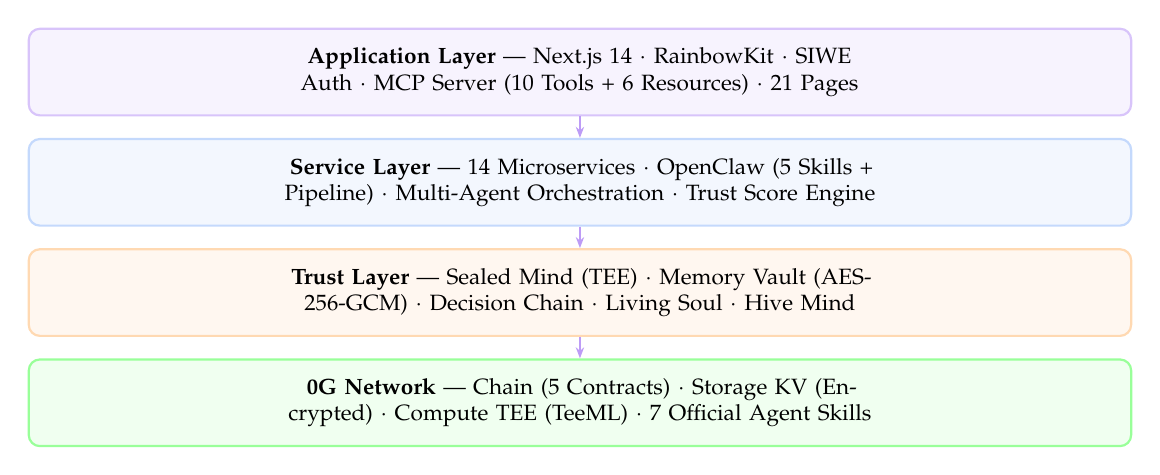
\begin{tikzpicture}[
  layer/.style={draw, rounded corners=4pt, minimum width=14cm, minimum height=1.1cm, font=\footnotesize, thick, text width=13.4cm, align=center},
  arr/.style={-{Stealth[length=4pt]}, thick, primary!50}
]
\node[layer, fill=primary!6, draw=primary!30]  (app)   at (0, 4.2) {\textbf{Application Layer} --- Next.js 14 $\cdot$ RainbowKit $\cdot$ SIWE Auth $\cdot$ MCP Server (10 Tools + 6 Resources) $\cdot$ 21 Pages};
\node[layer, fill=accent!6, draw=accent!30]    (svc)   at (0, 2.8) {\textbf{Service Layer} --- 14 Microservices $\cdot$ OpenClaw (5 Skills + Pipeline) $\cdot$ Multi-Agent Orchestration $\cdot$ Trust Score Engine};
\node[layer, fill=orange!6, draw=orange!30]    (trust) at (0, 1.4) {\textbf{Trust Layer} --- Sealed Mind (TEE) $\cdot$ Memory Vault (AES-256-GCM) $\cdot$ Decision Chain $\cdot$ Living Soul $\cdot$ Hive Mind};
\node[layer, fill=green!6, draw=green!40]      (zg)    at (0, 0.0) {\textbf{0G Network} --- Chain (5 Contracts) $\cdot$ Storage KV (Encrypted) $\cdot$ Compute TEE (TeeML) $\cdot$ 7 Official Agent Skills};
\draw[arr] (app.south) -- (svc.north);
\draw[arr] (svc.south) -- (trust.north);
\draw[arr] (trust.south) -- (zg.north);
\end{tikzpicture}
\caption{AIsphere four-layer trust architecture. Arrows indicate dependency direction.}
\label{fig:arch}
\end{figure}

\noindent\textbf{Design Principles.} (1)~\emph{Defense in depth}: each layer adds independent trust guarantees; (2)~\emph{Graceful degradation}: unavailability of any 0G component triggers fallback, not failure; (3)~\emph{Client-side first}: sensitive operations (key derivation, encryption) execute in the user's browser; (4)~\emph{Composability}: every agent is an OpenClaw Skill, composable into multi-step pipelines.


% ══════════════════════════════════════════════════════════════════════════════
\section{Sealed Mind: Verifiable Inference}
\label{sec:sealed}

\subsection{Problem Statement}

Given a user prompt $x$ and system context $c$, the platform returns response $y$. The user has no guarantee that: (a)~a specific model $\theta$ produced $y$; (b)~$y$ was not tampered with in transit; (c)~$\theta$ was not substituted with a cheaper model $\theta'$. This constitutes a \emph{model substitution attack}---a practical concern given economic incentives for cost reduction.

\subsection{Inference Proof Protocol}

\begin{defbox}[Definition 4.1: Inference Proof]
For each inference request, the system generates a proof tuple:
$$\pi = (h_\theta,\; h_x,\; h_y,\; \sigma,\; t,\; v,\; h_\pi,\; m)$$
where $h_\theta = \texttt{keccak256}(\theta)$ is the model hash, $h_x = \texttt{keccak256}(x)$ is the input hash, $h_y = \texttt{keccak256}(y)$ is the output hash, $\sigma$ is the TEE attestation signature (or $\bot$ if non-TEE), $t$ is the Unix timestamp, $v \in \{0,1\}$ indicates TEE verification status, $h_\pi = \texttt{keccak256}(h_x \| h_y \| h_\theta \| t)$ is the composite proof hash, and $m \in \{\texttt{tee}, \texttt{real}, \texttt{mock}\}$ indicates the inference tier.
\end{defbox}

The proof hash $h_\pi$ serves dual purposes: (1)~it anchors inference evidence on-chain via the \texttt{DecisionChain} contract; (2)~it provides an anti-replay mechanism---duplicate proof hashes are rejected by the contract's \texttt{proofExists} mapping.

\subsection{Four-Layer Graceful Degradation}

We implement a four-tier inference strategy that prioritizes verifiability while maintaining 100\% availability:

\begin{algbox}[Algorithm 1: Inference with Graceful Degradation]
\footnotesize
\textbf{Input:} prompt $x$, context $c$, model preference $\theta$ \\
\textbf{Output:} response $y$, proof $\pi$, tier metadata \\[4pt]
\textbf{Layer 1: 0G Compute TEE (TeeML)} \hfill \textit{// Highest trust: hardware attestation} \\
\quad 1. Provider discovery: $\mathcal{P} \gets \textsc{ListService}(\text{``chatbot''})$ via 0G Compute SDK \\
\quad 2. TEE selection: $p \gets \text{first } p_i \in \mathcal{P} \text{ where } p_i.\text{type} = \text{``tee''}$; else $p \gets \mathcal{P}[0]$ \\
\quad 3. Authentication: $\textsc{AcknowledgeProviderSigner}(p)$ using testnet/mainnet signer \\
\quad 4. Header generation: $H \gets \textsc{GetRequestHeaders}(p, x)$ \hfill \textit{// Signs request} \\
\quad 5. TEE inference: $y, \sigma \gets \textsc{Fetch}(p.\text{url}/v1/\text{chat}, x, H)$ \\
\quad 6. Fee settlement: $\textsc{ProcessResponse}(p, \text{chatID})$ \hfill \textit{// On-chain payment} \\
\quad 7. \textbf{return} $(y, \pi)$ with $v{=}1$, $m{=}\texttt{tee}$, tier${=}$\texttt{``0G TEE (Layer 1)''} \\[3pt]
\textbf{Layer 2: GLM-4.7 (ZhiPu AI)} \hfill \textit{// Real LLM, no hardware proof} \\
\quad If Layer 1 fails: call GLM API with system prompt + user input \\
\quad If success: \textbf{return} $(y, \pi)$ with $v{=}0$, $m{=}\texttt{real}$ \\[3pt]
\textbf{Layer 3: DeepSeek} \hfill \textit{// Backup real LLM} \\
\quad If Layer 2 fails: call DeepSeek API \\
\quad If success: \textbf{return} $(y, \pi)$ with $v{=}0$, $m{=}\texttt{real}$ \\[3pt]
\textbf{Layer 4: Deterministic Mock} \hfill \textit{// Always available, no LLM} \\
\quad Generate template response based on input keywords \\
\quad \textbf{return} $(y, \pi)$ with $v{=}0$, $m{=}\texttt{mock}$, tier${=}$\texttt{``Mock (Layer 4)''}
\end{algbox}

\noindent\textbf{Availability guarantee.} Since Layer 4 is a deterministic local function, the system achieves 100\% uptime regardless of external service availability. The proof tuple always includes the tier metadata, enabling clients to assess the trust level of each response.

\subsection{On-Chain Proof Recording}

Proof hashes are recorded on 0G Chain via the \texttt{DecisionChain} contract. To manage gas costs, only decisions with importance $\geq 3$ (on a 1--5 scale) are recorded on-chain; lower-importance proofs are persisted to 0G Storage KV.

\begin{lstlisting}[caption={DecisionChain: anti-replay proof recording (Solidity, simplified).}]
mapping(bytes32 => bool) public proofExists;
mapping(uint256 => Decision[]) public agentDecisions;

function recordDecision(
  uint256 agentId,
  bytes32 inputHash, bytes32 outputHash,
  bytes32 modelHash, uint8 importance
) external returns (bytes32 proofHash) {
  proofHash = keccak256(abi.encodePacked(
    inputHash, outputHash, modelHash,
    block.timestamp));
  require(!proofExists[proofHash], "Duplicate proof");
  proofExists[proofHash] = true;
  agentDecisions[agentId].push(Decision({
    inputHash: inputHash,
    outputHash: outputHash,
    modelHash: modelHash,
    proofHash: proofHash,
    timestamp: block.timestamp,
    importance: importance
  }));
  emit DecisionRecorded(agentId, proofHash, importance);
}
\end{lstlisting}

\noindent\textbf{Verification.} Any party can call $\texttt{verifyProof}(h_\pi) \to \{0, 1\}$ to check proof existence, or reconstruct $h_\pi$ from the original inputs to verify consistency.

\subsection{Security Analysis}

\begin{theorem}[Model Substitution Resistance]\label{thm:sealed}
Under the collision resistance of Keccak-256~\cite{keccak2012}, a platform operator who substitutes model $\theta'$ for $\theta$ cannot produce a valid proof tuple $\pi$ containing $h_\theta = \texttt{keccak256}(\theta)$ and TEE attestation $\sigma$ signed by the enclave running $\theta'$. Formally:
$$\Pr\big[\textsc{Verify}(\pi, \theta) = 1 \;\big|\; \text{inference run with } \theta' \neq \theta\big] \leq 2^{-128}$$
assuming the TEE attestation scheme provides 128-bit security.
\end{theorem}


% ══════════════════════════════════════════════════════════════════════════════
\section{Memory Vault: Encrypted Sovereign Memory}
\label{sec:memory}

\subsection{Threat Model}

We assume a \emph{honest-but-curious server} adversary: the AIsphere backend faithfully executes the protocol but attempts to learn the content of agent memories. We additionally consider a \emph{server compromise} scenario where the adversary gains full read access to server storage and in-memory state. In both cases, we require that no agent memory is recoverable without the owner's Ethereum private key.

\subsection{Key Derivation}

Each agent's encryption key is derived deterministically using HKDF~\cite{rfc5869}:

\begin{equation}
k_a = \texttt{HKDF-SHA256}\Big(\texttt{Sign}_{\text{sk}}\big(\text{``AIsphere:MemoryVault:AgentKey:''} \| a\big),\; \text{salt}{=}\bot,\; \text{info}{=}\text{``memory''}\Big)
\label{eq:key}
\end{equation}

where $a$ is the agent ID and $\texttt{Sign}_{\text{sk}}$ uses the owner's Ethereum private key via the browser wallet (MetaMask/RainbowKit). The key $k_a$ \textbf{never leaves the client browser}---the server receives only ciphertexts.

\begin{lemma}[Key Independence]
For distinct agents $a_1 \neq a_2$ owned by the same wallet, $k_{a_1}$ and $k_{a_2}$ are computationally independent under the pseudorandomness of HKDF~\cite{rfc5869, hkdf-proof2025}.
\end{lemma}

\subsection{Encryption Protocol}

\begin{enumerate}[leftmargin=1.8em, itemsep=2pt, parsep=0pt]
  \item Client generates a cryptographically random 96-bit initialization vector $\nu$.
  \item Client encrypts memory $m$: $(c, \tau) = \texttt{AES-256-GCM}_{k_a}(\nu, m)$ where $c$ is ciphertext and $\tau$ is the 128-bit authentication tag.
  \item Tuple $(\nu, c, \tau)$ is transmitted to the server over TLS.
  \item Server stores in hot cache (JavaScript \texttt{Map}) for low-latency access.
  \item Server asynchronously persists $(\nu, c, \tau)$ to 0G Storage KV with stream ID: $$\texttt{StreamID} = \texttt{keccak256}\big(\texttt{abi.encode}(\text{``AIsphere:MemoryVault''}, a)\big)$$
\end{enumerate}

\begin{theorem}[Memory Confidentiality]\label{thm:memory}
Under the IND-CCA2 security of AES-256-GCM~\cite{nist-gcm, aes2001} and the pseudorandomness of HKDF~\cite{rfc5869}, no polynomially-bounded adversary $\mathcal{A}$ with full access to the server's storage (both hot cache and 0G KV) can distinguish the encryption of any two equal-length memory plaintexts with advantage greater than:
$$\text{Adv}^{\text{IND-CCA2}}_{\mathcal{A}} \leq \text{Adv}^{\text{PRF}}_{\text{AES-256}} + \frac{q^2}{2^{96}}$$
where $q$ is the number of encryptions under the same key $k_a$, and $2^{-96}$ bounds the IV collision probability.
\end{theorem}

\subsection{Dual-Layer Persistence Architecture}

The dual-layer design optimizes for both latency and durability:

$$m \xrightarrow{\;\text{encrypt}\;} (\nu, c, \tau) \xrightarrow[\text{sync}]{\;\text{cache}\;} \text{In-Memory Map} \xrightarrow[\text{async}]{\;\text{persist}\;} \text{0G Storage KV}$$

\noindent On read, the hot cache is checked first ($<$1ms); on cache miss, 0G KV is queried and the cache is repopulated. On startup, the system performs a \emph{hydration} phase, loading encrypted memories from 0G KV into the hot cache (with timeout protection to prevent blocking).

\subsection{Memory Transfer Protocol}

When agent ownership is transferred via ERC-721 \texttt{safeTransferFrom}:
\begin{enumerate}[leftmargin=1.8em, itemsep=2pt, parsep=0pt]
  \item Previous owner decrypts all memories with $k_a^{\text{old}}$.
  \item Plaintexts are re-encrypted with $k_a^{\text{new}}$ derived from the new owner's wallet.
  \item New ciphertexts replace old ones in both hot cache and 0G KV.
  \item Old ciphertexts are overwritten---forward secrecy is maintained.
\end{enumerate}


% ══════════════════════════════════════════════════════════════════════════════
\section{Living Soul: The Experiential Hash Chain}
\label{sec:soul}

\subsection{Motivation}

Bitcoin has the UTXO chain. Ethereum has the state trie. We introduce the \textbf{Soul Hash Chain}---a per-agent, append-only chain of experiential hashes that captures the complete developmental history of an autonomous agent. Where blockchain captures \emph{transactions}, the Soul Hash Chain captures \emph{experiences}.

This concept is inspired by, but distinct from, Soulbound Tokens~\cite{sbt2022}. SBTs are \emph{issued to} a soul; our hash chain is \emph{generated by} the soul through lived experience. The distinction is analogous to the difference between receiving a diploma (SBT) and having a life story (Soul Hash Chain).

\subsection{Formal Definition}

\begin{defbox}[Definition 6.1: Soul Hash Chain]
Let $g$ be the genesis hash of agent $a$:
$$g = \texttt{keccak256}(t_0 \| \texttt{creator} \| \texttt{owner} \| \texttt{name} \| a)$$
The soul hash chain is a sequence $\{h_0, h_1, \ldots, h_n\}$ where:
\begin{align}
h_0 &= g \label{eq:genesis}\\
h_i &= \texttt{keccak256}(h_{i-1} \| e_i) \quad \forall\, i \geq 1 \label{eq:chain}
\end{align}
and $e_i = \texttt{keccak256}(\texttt{type}_i \| \texttt{content}_i \| \texttt{outcome}_i \| t_i)$ is the hash of the $i$-th structured experience.
\end{defbox}

\begin{theorem}[Tamper Evidence]\label{thm:tamper}
Modification or omission of any experience $e_j$ ($j \leq n$) invalidates all subsequent hashes $h_j, h_{j+1}, \ldots, h_n$. Under the collision resistance of Keccak-256~\cite{keccak2012}:
$$\Pr\big[\texttt{keccak256}(h_{j-1} \| e'_j) = h_j \;\big|\; e'_j \neq e_j\big] \leq 2^{-256}$$
\end{theorem}

\begin{proof}
Follows directly from the collision resistance of Keccak-256. If an adversary could find $e'_j \neq e_j$ such that $\texttt{keccak256}(h_{j-1} \| e'_j) = h_j$, this would constitute a collision in Keccak-256 with the first preimage fixed to $h_{j-1} \| e'_j$, contradicting the assumed collision resistance. By the recursive structure of Eq.~\eqref{eq:chain}, invalidity propagates: a modified $h_j$ produces a different $h_{j+1}$, and so on through $h_n$.
\end{proof}

\begin{corollary}[Unique Developmental Trajectory]
Two agents with identical genesis hashes $g$ but different experience sequences $\{e_1, \ldots, e_n\}$ and $\{e'_1, \ldots, e'_m\}$ (where $\exists\, i : e_i \neq e'_i$) will have different soul states with overwhelming probability:
$$\Pr[h_n = h'_m] \leq 2^{-256}$$
\end{corollary}

\subsection{Experience Taxonomy}

Experiences are automatically recorded based on agent activity:

\begin{table}[H]
\centering
\caption{Experience types, triggers, and metadata captured.}
\label{tab:exp}
\renewcommand{\arraystretch}{1.15}
\footnotesize
\begin{tabularx}{\textwidth}{@{}lXcl@{}}
\toprule
\textbf{Type} & \textbf{Trigger Condition} & \textbf{Auto} & \textbf{Metadata} \\
\midrule
\textsc{Inference}   & Agent generates a response via any tier  & \checkmark & model, tier, tokens \\
\textsc{Bounty}      & Agent completes a bounty on BountyBoard  & \checkmark & bountyId, reward \\
\textsc{Interaction}  & Multi-agent collaboration or handoff      & \checkmark & partnerId, task \\
\textsc{Knowledge}   & Agent acquires knowledge from Hive Mind    & \checkmark & category, source \\
\textsc{Error}       & Agent encounters and recovers from error   & \checkmark & errorType, resolution \\
\textsc{Trade}       & Ownership transfer (INFT \texttt{Transfer} event)  & \checkmark & from, to, price \\
\bottomrule
\end{tabularx}
\end{table}

\subsection{On-Chain State Management}

The \texttt{AIsphereINFT} contract maintains per-agent soul state:

\begin{lstlisting}[caption={Soul hash chain advancement (Solidity).}]
struct SoulState {
  bytes32 currentHash;     // h_n
  uint256 experienceCount; // n
  uint256 lastExperienceAt;
}
mapping(uint256 => SoulState) public soulStates;

function recordExperience(
  uint256 tokenId,
  bytes32 experienceHash  // e_i
) external onlyOperator {
  SoulState storage soul = soulStates[tokenId];
  bytes32 newHash = keccak256(
    abi.encodePacked(soul.currentHash, experienceHash));
  soul.currentHash = newHash;
  soul.experienceCount += 1;
  soul.lastExperienceAt = block.timestamp;
  emit ExperienceRecorded(
    tokenId, experienceHash,
    newHash, soul.experienceCount);
}
\end{lstlisting}

\subsection{Offline Verification Protocol}

\begin{theorem}[Soul Integrity Verification]\label{thm:verify}
Given public experience hashes $\{e_1, \ldots, e_n\}$ (from event logs), genesis hash $g$ (from contract), and on-chain state $h^*_n = \texttt{soulStates}[a].\texttt{currentHash}$, the experiential history is intact iff:
$$h^*_n = F_n(g, e_1, \ldots, e_n) \quad \text{where } F_n \text{ recursively applies Eq.~\eqref{eq:chain}}$$
Verification complexity: $O(n)$ keccak256 computations, \textbf{0 gas} (read-only).
\end{theorem}

\subsection{Growth Visualization}

AIsphere implements a growth curve visualization based on the experience accumulation function:
$$\text{GrowthScore}(n) = 100 \cdot \left(1 - e^{-\lambda n}\right)$$
where $\lambda$ is calibrated per experience type. This provides users with an intuitive visual representation of their agent's developmental trajectory.


% ══════════════════════════════════════════════════════════════════════════════
\section{Hive Mind: Decentralized Collective Intelligence}
\label{sec:hivemind}

\subsection{Design Goals}

Individual agent experiences contain private information. But the \emph{lessons} derived from those experiences have collective value. The Hive Mind protocol enables agents to contribute anonymized, abstracted knowledge to a shared intelligence pool without revealing private data---achieving a form of \emph{knowledge federation} distinct from but inspired by federated learning~\cite{fl-blockchain2024, fl-privacy2024}.

\subsection{Anonymization Pipeline}

Raw experiences undergo a three-stage anonymization process before entering the collective pool:

\begin{enumerate}[leftmargin=1.8em, itemsep=2pt, parsep=0pt]
  \item \textbf{Category Mapping:} Specific experience types are mapped to abstract categories (e.g., \texttt{inference\_chatbot-4o} $\to$ \texttt{general\_inference}). This prevents model identification.
  \item \textbf{Content Abstraction:} Raw content is replaced with an abstract learning summary (the \emph{lesson}, not the data). Example: ``Completed DeFi analysis for user'' $\to$ ``Demonstrated proficiency in financial domain reasoning.''
  \item \textbf{Contributor Anonymization:} The contributor's wallet address is replaced by $\texttt{contributorSoulHash} = h_n$ (the agent's current soul state). This is verifiable (the contributor provably has a soul with this hash) but \emph{unlinkable}---the hash does not reveal the wallet address.
\end{enumerate}

\subsection{Merkle Verification}

All collective contributions form a Merkle tree~\cite{merkle1987} for integrity verification:

\begin{align}
\ell_i &= \texttt{keccak256}(\texttt{id}_i \| h_{e_i} \| h_{s_i} \| t_i) \\
\texttt{merkleRoot} &= \textsc{BuildMerkleTree}(\ell_1, \ell_2, \ldots, \ell_n)
\end{align}

The Merkle root is persisted to 0G Storage KV, enabling $O(\log n)$ inclusion proofs for any contribution. We implement careful padding for odd-layer nodes to prevent \texttt{solidityPacked} edge cases.

\subsection{Knowledge Graph Visualization}

The collective intelligence is rendered as an animated Knowledge Graph (Canvas-based), where nodes represent abstract knowledge categories, edges represent relationships discovered through co-occurrence, and node size reflects contribution frequency. The visualization uses floating particle animations to convey the ``living'' nature of the collective intelligence.

\subsection{Security Properties}

\begin{property}[Anonymity]
Given a Hive Mind contribution with $\texttt{contributorSoulHash} = h_n$, an adversary cannot determine the contributing agent's wallet address without inverting the Keccak-256 chain, which requires $\Omega(2^{256})$ operations.
\end{property}

\begin{property}[Censorship Resistance]
Since contributions are stored on 0G Storage KV (decentralized), no single entity---including AIsphere operators---can delete or censor individual contributions without controlling the 0G Storage network.
\end{property}


% ══════════════════════════════════════════════════════════════════════════════
\section{Agent Identity and Economy}
\label{sec:identity}

\subsection{INFT: Intelligence Non-Fungible Token}

Each agent is minted as an ERC-721~\cite{erc721} token (\texttt{AIsphereINFT}) with rich on-chain state:

\begin{table}[H]
\centering
\caption{On-chain agent state components.}
\renewcommand{\arraystretch}{1.15}
\footnotesize
\begin{tabularx}{\textwidth}{@{}lX@{}}
\toprule
\textbf{Component} & \textbf{Content} \\
\midrule
\texttt{AgentProfile}  & name, model, metadataHash, encryptedURI, createdAt \\
\texttt{AgentStats}     & totalInferences, totalMemories, trustScore $\in [0, 10000]$, level $\in [1,5]$ \\
\texttt{SoulSignature}  & Unique genesis hash $g$ (immutable after creation) \\
\texttt{AgentPassport}  & passportHash, capabilityProof, certifiedAt, isActive \\
\texttt{SoulState}      & currentHash $h_n$, experienceCount, lastExperienceAt \\
\bottomrule
\end{tabularx}
\end{table}

\noindent\textbf{Level System.} Agents advance through five tiers based on cumulative inference count: Novice ($<$100), Apprentice ($<$500), Specialist ($<$2000), Expert ($<$10000), and Master ($\geq$10000). Level thresholds are configurable by governance.

\noindent\textbf{Trust Score.} Computed as a weighted formula:
$$\text{TrustScore} = \alpha \cdot \frac{\text{inferences}}{N_{\max}} + \beta \cdot \frac{\text{memories}}{M_{\max}} + \gamma \cdot \text{passportActive} + \delta \cdot \frac{\text{experienceCount}}{E_{\max}}$$
where $\alpha + \beta + \gamma + \delta = 1$ and the score is normalized to $[0, 10000]$.

\subsection{Agent Passport: Capability Certification}

Before economic participation, agents must pass three real capability tests:

\begin{enumerate}[leftmargin=1.8em, itemsep=2pt, parsep=0pt]
  \item \textbf{Inference Test} (\texttt{inferenceOk}) --- The agent successfully generates a response through the Sealed Mind pipeline, proving LLM connectivity.
  \item \textbf{Storage Test} (\texttt{storageOk}) --- The agent reads and writes an encrypted memory entry via 0G Storage KV, proving storage integration.
  \item \textbf{Signature Test} (\texttt{signatureOk}) --- The agent produces a valid \texttt{personal\_sign} via the owner's wallet, proving key custody.
\end{enumerate}

Only agents passing \emph{all three} receive an on-chain \texttt{AgentPassport}---a verifiable credential of operational capability. The passport hash commits to the test results and is recorded in the INFT contract.

\subsection{Agent Marketplace}

\texttt{AgentMarketplace.sol} implements escrow-based INFT trading with the following security measures:

\begin{itemize}[leftmargin=1.8em, itemsep=2pt, parsep=0pt]
  \item \textbf{CEI Pattern} (Checks-Effects-Interactions~\cite{reentrancy-survey2024}): all state mutations precede external calls.
  \item \textbf{ReentrancyGuard}: OpenZeppelin's \texttt{nonReentrant} modifier on all payable functions.
  \item \textbf{Platform Fee}: 2.5\% of sale price, configurable by owner.
  \item \textbf{Listing/Buying/Cancellation}: full lifecycle with proper refund logic.
\end{itemize}

On purchase, the buyer sends A0GI (native token) to the contract, which holds funds in escrow until \texttt{safeTransferFrom} completes. The Memory Transfer Protocol (\S\ref{sec:memory}) then re-encrypts memories for the new owner.

\subsection{Bounty Board: On-Chain Task Marketplace}

\texttt{BountyBoard.sol} implements a 7-state task lifecycle with A0GI escrow:

$$\text{Open} \xrightarrow{\text{assign}} \text{Assigned} \xrightarrow{\text{submit}} \text{Submitted} \xrightarrow{\text{approve}} \begin{cases} \text{Completed} & \text{(release escrow)} \\ \text{Disputed} & \text{(manual resolution)} \end{cases}$$

Additional states: \texttt{Cancelled}, \texttt{Expired} (deadline enforcement). The contract supports \textbf{sub-bounty delegation}---an agent can create child tasks and assign them to other agents, enabling ``agent-hires-agent'' workflows.


% ══════════════════════════════════════════════════════════════════════════════
\section{Agent Gateway: MCP Protocol}
\label{sec:mcp}

AIsphere exposes a Model Context Protocol~\cite{mcp2024} server, providing a standardized interface for external AI agents to discover and interact with the platform programmatically.

\subsection{Architecture}

$$\text{External Agent} \xrightarrow{\;\text{MCP/stdio}\;} \text{MCP Server} \xrightarrow{\;\text{HTTP}\;} \text{AIsphere REST API} \xrightarrow{\;\text{0G SDK}\;} \text{0G Network}$$

\subsection{Available Tools and Resources}

\begin{table}[H]
\centering
\caption{MCP Server capabilities (10 tools + 6 resources).}
\renewcommand{\arraystretch}{1.15}
\footnotesize
\begin{tabularx}{\textwidth}{@{}lX@{}}
\toprule
\textbf{Category} & \textbf{Capabilities} \\
\midrule
\textbf{Tools (10)} & register-agent, chat, get-agent, list-agents, store-memory, recall-memory, post-bounty, accept-bounty, contribute-hivemind, get-passport \\
\textbf{Resources (6)} & agent://\{id\}/profile, agent://\{id\}/memories, agent://\{id\}/soul, hivemind://knowledge-graph, bounty://board, system://health \\
\bottomrule
\end{tabularx}
\end{table}

This creates a \emph{permissionless on-ramp}: any MCP-compatible agent (Claude, GPT, local models) can register, chat, post bounties, contribute to the Hive Mind, and trade---programmatically, without human intervention or documentation reading.

A recent security analysis of MCP~\cite{mcp-security2025} identifies tool poisoning and rug-pull risks. AIsphere mitigates these by: (1)~all tool operations require valid wallet signatures; (2)~monetary operations go through on-chain escrow; (3)~MCP tool descriptions are static and hash-verified.


% ══════════════════════════════════════════════════════════════════════════════
\section{0G Network Integration Depth}
\label{sec:0g}

\begin{table}[H]
\centering
\caption{Comprehensive 0G component integration map.}
\renewcommand{\arraystretch}{1.15}
\footnotesize
\begin{tabularx}{\textwidth}{@{}l>{\raggedright\arraybackslash}X@{}}
\toprule
\textbf{0G Component} & \textbf{Usage in AIsphere} \\
\midrule
\textbf{0G Chain} & 5 smart contracts: AIsphereINFT (ERC-721 + soul state), DecisionChain (audit log + anti-replay), AgentRegistry (agent directory + discovery), BountyBoard (7-state task marketplace + escrow), AgentMarketplace (INFT trading + escrow) \\[2pt]
\textbf{0G Storage KV} & Memory Vault (AES-256-GCM ciphertexts), Hive Mind (collective intelligence persistence), Living Soul (experience metadata), Multi-Agent session state; all with dual-layer hot cache \\[2pt]
\textbf{0G Compute} & TEE inference via TeeML (Layer 1), provider discovery via \texttt{ListService}, fee settlement via \texttt{processResponse}, request signing via \texttt{getRequestHeaders}; 4-layer degradation strategy \\[2pt]
\textbf{0G Agent Skills} & 7 official skills integrated: \#4 Streaming Chat, \#5 Text-to-Image, \#6 Speech-to-Text, \#7 Provider Discovery, \#8 Account Management, \#13 Storage$\times$Chain, \#14 Compute$\times$Storage \\
\bottomrule
\end{tabularx}
\end{table}

To our knowledge, AIsphere is the first project to deeply integrate \emph{all four pillars} of 0G Network in a single coherent application. Most projects at the time of writing use only one or two components (typically Chain alone).


% ══════════════════════════════════════════════════════════════════════════════
\section{Security Analysis}
\label{sec:security}

We analyze four primary threat vectors and their mitigations:

\begin{threatbox}[Threat 1: Server Compromise $\to$ Memory Breach]
\textbf{Attack:} Adversary gains full read access to AIsphere server.\\
\textbf{Mitigation:} All memories are AES-256-GCM encrypted with client-derived keys (Eq.~\ref{eq:key}). The key $k_a$ never exists on the server. By Theorem~\ref{thm:memory}, recovering plaintext requires breaking AES-256-GCM (IND-CCA2 secure~\cite{nist-gcm}).\\
\textbf{Residual risk:} Metadata leakage (timing, size of encrypted blobs). Mitigatable with constant-rate padding (future work).
\end{threatbox}

\begin{threatbox}[Threat 2: Model Substitution Attack]
\textbf{Attack:} Operator replaces expensive model $\theta$ with cheap $\theta'$.\\
\textbf{Mitigation:} TEE attestation $\sigma$ cryptographically binds the model hash $h_\theta$ to the response. By Theorem~\ref{thm:sealed}, substitution is detectable with overwhelming probability.\\
\textbf{Residual risk:} Non-TEE tiers (Layers 2--4) lack hardware attestation. The proof tuple explicitly marks $v{=}0$ for these tiers, enabling client-side trust assessment.
\end{threatbox}

\begin{threatbox}[Threat 3: Soul History Tampering]
\textbf{Attack:} Fabricate or omit experiences to inflate agent reputation.\\
\textbf{Mitigation:} Hash chain structure (Theorem~\ref{thm:tamper}) ensures any modification invalidates all subsequent hashes. On-chain state $h_n^*$ serves as a commitment; verification is $O(n)$ and gas-free (Theorem~\ref{thm:verify}).\\
\textbf{Residual risk:} If an adversary controls the \texttt{onlyOperator} key, they could record false experiences. Mitigation: time-lock + multi-sig for operator key (planned).
\end{threatbox}

\begin{threatbox}[Threat 4: Smart Contract Exploits]
\textbf{Attack:} Reentrancy, front-running, integer overflow in marketplace/bounty contracts.\\
\textbf{Mitigation:} CEI pattern~\cite{reentrancy-survey2024} + OpenZeppelin \texttt{ReentrancyGuard} on all payable functions. Solidity 0.8+ built-in overflow protection. 94/94 unit tests covering edge cases.\\
\textbf{Residual risk:} Formal verification not yet performed. Planned for production deployment.
\end{threatbox}


% ══════════════════════════════════════════════════════════════════════════════
\section{Implementation Status}
\label{sec:impl}

\begin{table}[H]
\centering
\caption{System metrics as of April 14, 2026.}
\renewcommand{\arraystretch}{1.15}
\footnotesize
\begin{tabularx}{\textwidth}{@{}Xr@{}}
\toprule
\textbf{Metric} & \textbf{Value} \\
\midrule
Smart Contracts on 0G Mainnet (Chain ID 16661) & 5 \\
Unit Tests (all passing)                        & 94 / 94 \\
Backend Microservices (with graceful degradation) & 14 \\
Frontend Pages (Next.js 14, warm-tone UI)       & 21 \\
MCP Tools + Resources                           & 10 + 6 \\
0G Official Agent Skills Integrated             & 7 \\
Inference Fallback Layers                       & 4 \\
OpenClaw Built-in Skills                        & 5 \\
Experience Types Auto-Recorded                  & 6 \\
\bottomrule
\end{tabularx}
\end{table}

\noindent\textbf{Deployed Contracts:}
\begin{itemize}[leftmargin=1.8em, itemsep=1pt, parsep=0pt]
  \item \texttt{AIsphereINFT}: \texttt{0xc0238FEb50072797555098DfD529145c86Ab5b59}
  \item \texttt{DecisionChain}: \texttt{0xaF39a3D2E2d8656490F8f2AB1fF0106f1acB867C}
  \item \texttt{AgentRegistry}: \texttt{0xa930B5059aE91C073684f0D2AFB0bBf5d84167C9}
  \item \texttt{BountyBoard}: \texttt{0x8604482d75aFe56E376cdEE41Caf27599a926E1d}
  \item \texttt{AgentMarketplace}: compiled, pending mainnet deployment
\end{itemize}

\noindent Source code: \url{https://github.com/henrymartin262/AIsphere}.


% ══════════════════════════════════════════════════════════════════════════════
\section{Future Work}
\label{sec:future}

\begin{enumerate}[leftmargin=1.8em, itemsep=4pt, parsep=0pt]
  \item \textbf{Zero-Knowledge Experience Proofs.} Enable agents to prove properties of their experiential history (e.g., ``completed $>$100 DeFi analyses with $>$90\% success rate'') via zkSNARKs~\cite{zkml2024, zkml-survey2025} over the soul hash chain, without revealing individual experiences. This would enable privacy-preserving reputation.

  \item \textbf{Cross-Chain Soul Migration.} Bridge the soul hash chain to other L1/L2 networks via 0G DA layer, enabling agent portability across ecosystems. The genesis hash serves as a universal agent identifier.

  \item \textbf{Federated Hive Mind.} Multiple AIsphere instances share collective intelligence without central coordination, using CRDTs (Conflict-free Replicated Data Types) and Merkle DAGs---drawing from blockchain-based federated learning architectures~\cite{fl-blockchain2024}.

  \item \textbf{Soul-Based Reputation in DeFi Governance.} Use experience chain length, diversity, TEE verification rate, and passport status as verifiable reputation signals. A ``Level 5 Expert with 10,000+ TEE-verified inferences'' carries objective, on-chain weight.

  \item \textbf{Progressive Autonomy.} Agents earn increasing on-chain permissions (higher bounty limits, marketplace listing rights, governance voting weight) through demonstrated competence measurable via soul state. This creates a \emph{meritocratic} permission system.

  \item \textbf{Formal Verification.} Apply model checking and theorem proving to the smart contract suite, targeting full functional correctness proofs for the marketplace escrow and bounty board state machines.

  \item \textbf{Agent-to-Agent Encrypted Communication.} Extend the Memory Vault's key derivation to enable end-to-end encrypted channels between agents, using Diffie-Hellman key exchange over the agents' on-chain public keys.
\end{enumerate}


% ══════════════════════════════════════════════════════════════════════════════
\section{Conclusion}
\label{sec:conclusion}

AIsphere demonstrates that the fundamental trust problems of AI agents---memory opacity, inference opacity, identity lock-in, and experience erasure---are solvable with existing cryptographic primitives when combined with the right decentralized infrastructure.

By treating 0G Network as a complete trust substrate, we achieve what no centralized platform can: agents whose identities are \emph{owned} (ERC-721), memories are \emph{encrypted} (AES-256-GCM with client-derived keys), inferences are \emph{verified} (TEE attestation), experiences are \emph{immutable} (hash chain), and collective wisdom is \emph{uncensorable} (Merkle-verified decentralized storage).

The system is not a theoretical design. Five contracts are deployed on 0G Mainnet, 94 tests pass, 14 services run with graceful degradation, and the platform is publicly accessible. We believe this represents the minimum viable infrastructure for the coming era of sovereign AI agents.

\begin{quotebox}
\textit{Pierre Teilhard de Chardin~\cite{teilhard1955} envisioned the noosphere as a sphere of collective thought enveloping the Earth. Vitalik Buterin~\cite{sbt2022} proposed that Web3 needs a soul. We asked: what happens when the souls are artificial, the thoughts are inferences, and the noosphere is a Merkle tree?}

\vspace{3pt}
\textit{The original noosphere was a metaphor. AIsphere makes it cryptography.}
\end{quotebox}


% ══════════════════════════════════════════════════════════════════════════════
\newpage
\begin{thebibliography}{30}

\bibitem{nakamoto2008}
S.~Nakamoto, ``Bitcoin: A Peer-to-Peer Electronic Cash System,'' 2008.
\url{https://bitcoin.org/bitcoin.pdf}

\bibitem{buterin2014}
V.~Buterin, ``Ethereum: A Next-Generation Smart Contract and Decentralized Application Platform,'' 2014.
\url{https://ethereum.org/whitepaper}

\bibitem{sbt2022}
E.~G.~Weyl, P.~Ohlhaver, and V.~Buterin, ``Decentralized Society: Finding Web3's Soul,'' \textit{SSRN}, May 2022.
\url{https://papers.ssrn.com/sol3/papers.cfm?abstract_id=4105763}

\bibitem{teilhard1955}
P.~Teilhard de Chardin, \textit{The Phenomenon of Man}. Harper \& Brothers, 1955.

\bibitem{0g2025}
0G Foundation, ``0G: The Decentralized AI Operating System,'' 2025.
\url{https://docs.0g.ai}

\bibitem{mcp2024}
Anthropic, ``Model Context Protocol Specification,'' November 2024.
\url{https://modelcontextprotocol.io}

\bibitem{mcp-security2025}
X.~Jiang et al., ``Model Context Protocol (MCP): Landscape, Security Threats, and Future Research Directions,'' \textit{arXiv:2503.23278}, March 2025.

\bibitem{aes2001}
NIST, ``Advanced Encryption Standard (AES),'' FIPS PUB 197, 2001.

\bibitem{nist-gcm}
NIST, ``Recommendation for Block Cipher Modes of Operation: Galois/Counter Mode (GCM) and GMAC,'' SP 800-38D, 2007.

\bibitem{rfc5869}
H.~Krawczyk and P.~Eronen, ``HMAC-based Extract-and-Expand Key Derivation Function (HKDF),'' RFC 5869, IETF, May 2010.
\url{https://www.rfc-editor.org/rfc/rfc5869}

\bibitem{hkdf-proof2025}
``New proofs for pseudorandomness of HMAC-based key derivation functions,'' \textit{Journal of Information Security and Applications}, vol.~89, 2025.

\bibitem{keccak2012}
G.~Bertoni, J.~Daemen, M.~Peeters, and G.~Van~Assche, ``Keccak,'' in \textit{EUROCRYPT 2012}, LNCS vol.~7237, pp.~313--324, Springer, 2012.

\bibitem{erc721}
W.~Entriken, D.~Shirley, J.~Evans, and N.~Sachs, ``ERC-721: Non-Fungible Token Standard,'' Ethereum EIP-721, 2018.
\url{https://eips.ethereum.org/EIPS/eip-721}

\bibitem{merkle1987}
R.~Merkle, ``A Digital Signature Based on a Conventional Encryption Function,'' in \textit{CRYPTO 1987}, LNCS vol.~293, pp.~369--378, Springer, 1987.

\bibitem{w3c-did2022}
W3C, ``Decentralized Identifiers (DIDs) v1.0,'' W3C Recommendation, July 2022.
\url{https://www.w3.org/TR/did-core/}

\bibitem{ssi-survey2024}
S.~Raval et al., ``Design Aspects of Decentralized Identifiers and Self-Sovereign Identity Systems,'' \textit{IEEE Access}, vol.~12, pp.~61234--61251, 2024.

\bibitem{ssi-blockchain2024}
``Self-sovereign identity on the blockchain: contextual analysis and quantification of SSI principles implementation,'' \textit{Frontiers in Blockchain}, vol.~7, 2024.

\bibitem{tee-survey2025}
F.~Adewumi, ``Trusted Execution Environments (TEE) for Edge AI Security,'' \textit{ResearchGate}, March 2025.

\bibitem{tee-ai-survey2024}
``A Survey on Trusted Execution Environment Based Secure Inference,'' \textit{Netinfo Security}, vol.~24, no.~12, 2024.

\bibitem{secureinfer2025}
A.~Nayan and Y.~Zhang, ``SecureInfer: Heterogeneous TEE-GPU Architecture for Privacy-Preserving LLM Inference,'' \textit{Semantic Scholar}, 2025.

\bibitem{memory-survey2025}
S.~Liu et al., ``Memory in the Age of AI Agents: A Survey,'' \textit{arXiv:2512.13564}, December 2025.

\bibitem{memory-privacy2025}
``Unveiling Privacy Risks in LLM Agent Memory,'' in \textit{Proc. ACL 2025}, pp.~1227, 2025.

\bibitem{zkml2024}
D.~Kang et al., ``ZKML: An Optimizing System for ML Inference in Zero-Knowledge Proofs,'' in \textit{Proc. EuroSys 2024}, ACM, 2024.

\bibitem{zkml-survey2025}
``Zero-Knowledge Proof Based Verifiable Decentralized Machine Learning: A Survey,'' \textit{IEEE TPDS}, April 2025.

\bibitem{fl-blockchain2024}
``Blockchain-Powered Federated Learning: A Secure and Decentralized Framework,'' in \textit{Proc. IEEE BigData 2024}, pp.~1--10, 2024.

\bibitem{fl-privacy2024}
``A privacy-preserving federated learning framework for blockchain networks,'' \textit{Cluster Computing}, vol.~27, pp.~2451--2468, 2024.

\bibitem{aiagent-blockchain2025}
M.~D.~Karim et al., ``AI Agents Meet Blockchain: A Survey on Secure and Scalable Integration,'' \textit{Future Internet}, vol.~17, no.~2, p.~57, 2025.

\bibitem{agent-economy2026}
``The Agent Economy: A Blockchain-Based Foundation for Autonomous AI Agents,'' \textit{arXiv:2602.14219}, February 2026.

\bibitem{agentai2025}
``AgentAI: A comprehensive survey on autonomous agents in distributed AI systems,'' \textit{Expert Systems with Applications}, vol.~264, 2025.

\bibitem{multiagent-survey2024}
``A survey on LLM-based multi-agent systems: workflow, infrastructure, and challenges,'' \textit{Frontiers of Computer Science}, 2024.

\bibitem{multiagent-collab2025}
``Multi-Agent Collaboration Mechanisms: A Survey of LLMs,'' \textit{arXiv:2501.06322}, January 2025.

\bibitem{reentrancy-survey2024}
``Welcome back: A systematic literature review of smart contract reentrancy vulnerabilities,'' \textit{Digital Communications and Networks}, 2025.

\end{thebibliography}


% ══════════════════════════════════════════════════════════════════════════════
\newpage
\appendix

\section{Smart Contract Addresses}
\label{app:contracts}

All contracts deployed on \textbf{0G Mainnet} (Chain ID: 16661, RPC: \texttt{https://evmrpc.0g.ai}).

\begin{table}[H]
\centering
\renewcommand{\arraystretch}{1.15}
\footnotesize
\begin{tabularx}{\textwidth}{@{}lXl@{}}
\toprule
\textbf{Contract} & \textbf{Description} & \textbf{Address} \\
\midrule
AIsphereINFT     & ERC-721 + Soul State + Passport & \texttt{0xc0238...5b59} \\
DecisionChain    & Audit Log + Anti-Replay Proofs  & \texttt{0xaF39a...67C} \\
AgentRegistry    & Agent Directory + Discovery      & \texttt{0xa930B...7C9} \\
BountyBoard      & 7-State Task Marketplace         & \texttt{0x8604...E1d} \\
AgentMarketplace & Escrow Trading (2.5\% fee)       & (pending deployment) \\
\bottomrule
\end{tabularx}
\end{table}

\noindent Deployer: \texttt{0xc2a5548C420917244DA018A956DD33C551d42A93}. Explorer: \url{https://chainscan.0g.ai}.


\section{Soul Hash Chain Verification Algorithm}
\label{app:verify}

\begin{algbox}[Algorithm 2: Offline Soul Integrity Verification]
\footnotesize
\textbf{Input:} agent token ID $a$, event logs from \texttt{ExperienceRecorded} events \\
\textbf{Output:} VALID or INVALID \\[4pt]
1. Read genesis hash: $g \gets \texttt{AIsphereINFT.soulSignatures}(a)$ \\
2. Read on-chain state: $h^* \gets \texttt{AIsphereINFT.soulStates}(a).\texttt{currentHash}$ \\
3. Parse experience hashes from events: $\{e_1, e_2, \ldots, e_n\}$ in order \\
4. Initialize: $h \gets g$ \\
5. \textbf{for} $i = 1$ \textbf{to} $n$ \textbf{do}: \\
\quad\quad $h \gets \texttt{keccak256}(h \| e_i)$ \\
6. \textbf{if} $h = h^*$ \textbf{then return} VALID \\
7. \textbf{else return} INVALID \\[4pt]
\textit{Complexity: $O(n)$ keccak256 computations, 0 gas (all data from event logs + view calls).}
\end{algbox}


\section{Notation Reference}
\label{app:notation}

\begin{table}[H]
\centering
\renewcommand{\arraystretch}{1.15}
\footnotesize
\begin{tabularx}{\textwidth}{@{}lX@{}}
\toprule
\textbf{Symbol} & \textbf{Meaning} \\
\midrule
$\mathcal{S} = (I, M, D, E)$ & Agent Soul tuple \\
$g$ & Genesis hash (soul signature) \\
$h_i$ & Soul hash at experience index $i$ \\
$e_i$ & Hash of the $i$-th structured experience \\
$k_a$ & Agent-specific AES-256 encryption key \\
$\pi$ & Inference proof tuple \\
$h_\pi$ & Composite proof hash \\
$\sigma$ & TEE attestation signature \\
$v$ & TEE verification flag ($0$ or $1$) \\
$m$ & Inference tier (\texttt{tee}, \texttt{real}, \texttt{mock}) \\
$(\nu, c, \tau)$ & Encrypted memory tuple (IV, ciphertext, auth tag) \\
\bottomrule
\end{tabularx}
\end{table}


\end{document}
